\documentclass{beamer}
\usetheme{Warsaw}

\usepackage{default}
\usepackage[utf8]{inputenc}
\usepackage[T1]{fontenc}
\usepackage{booktabs}
\usepackage{tikz}
\usepackage{listings}
\usepackage[english]{babel}
\usepackage{inconsolata}

\lstset{numbers=left, numberstyle=\tiny, basicstyle=\ttfamily, breaklines=true, tabsize=2, language=Python}

\author{András Veres-Szentkirályi}
\title{Extending Python Web Services}
\date{2012. január 20.}

\begin{document}

\frame{\titlepage}

\begin{frame}{Table of contents}
\tableofcontents
\end{frame}

\section{Environment}

\subsection{SOAP}

\begin{frame}
\begin{center}
 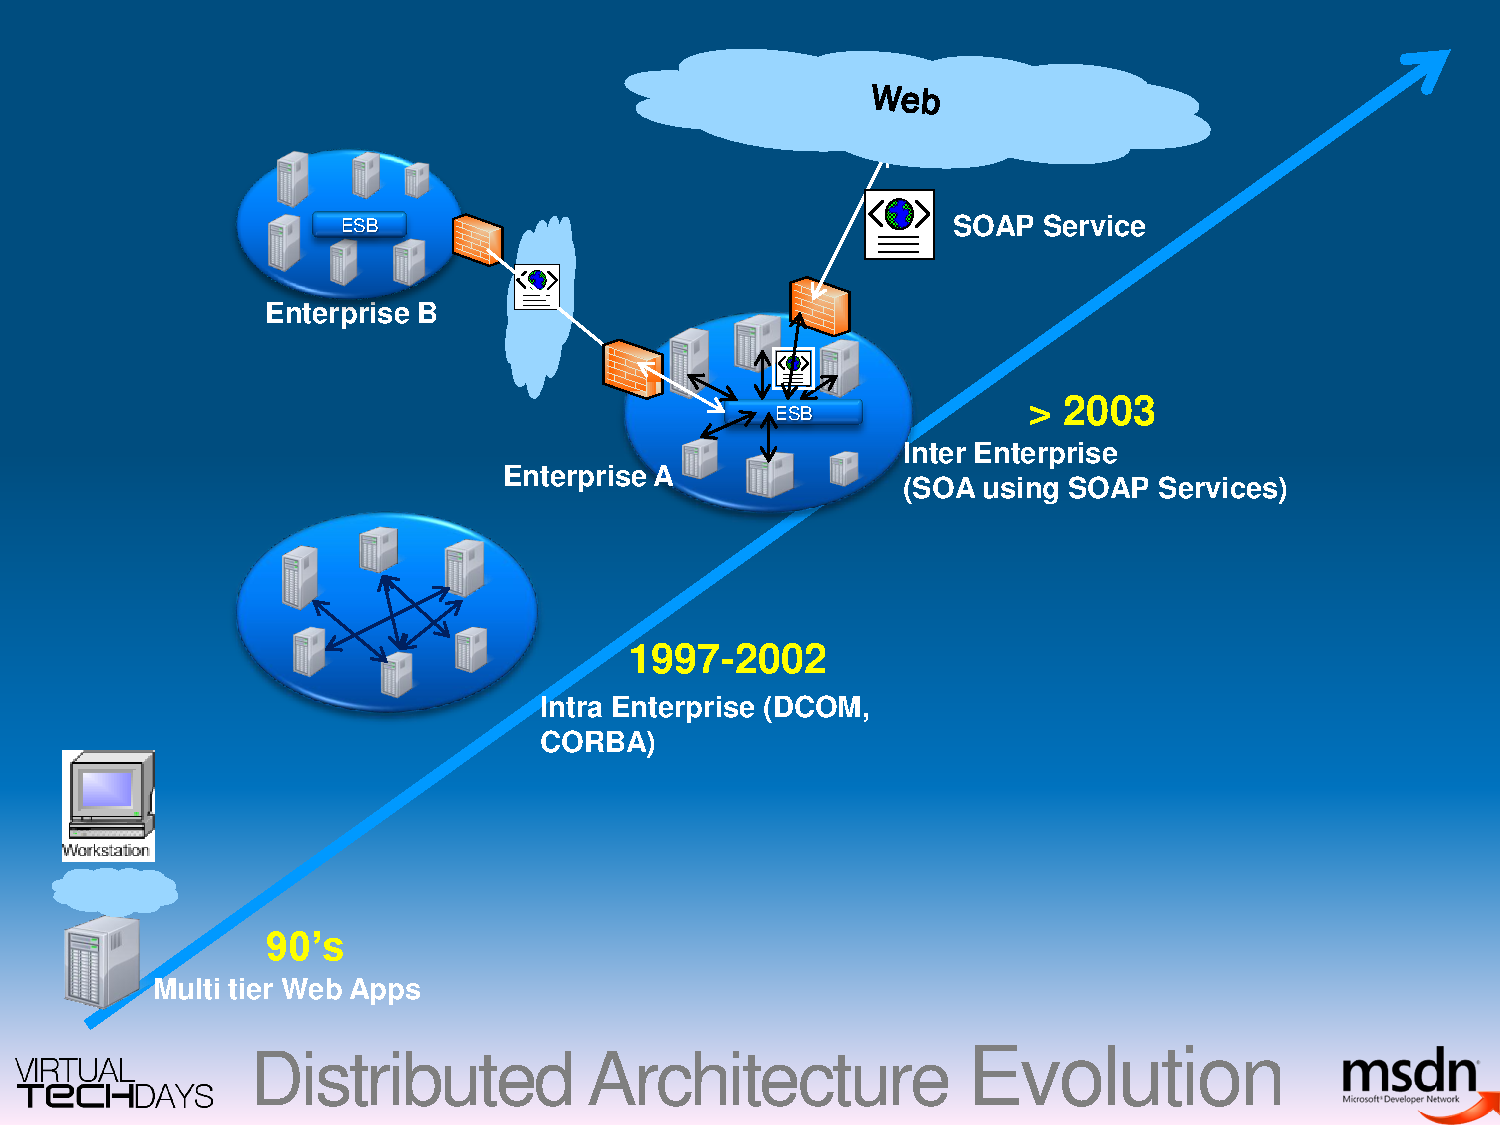
\includegraphics[height=7.5cm]{images/msdn-soap.pdf}
\end{center}
\end{frame}

\subsection{Python}

\begin{frame}
\begin{center}
 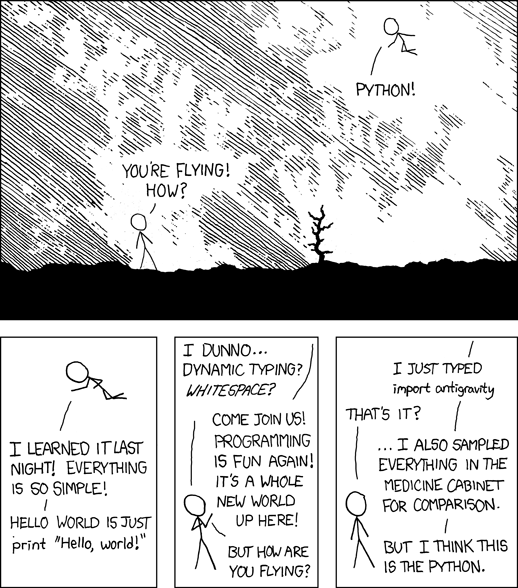
\includegraphics[height=7.5cm]{images/python.png}
\end{center}
\end{frame}

\subsection{WSSE}

\begin{frame}
\begin{center}
 
\includegraphics[height=7.5cm]{images/WSSE-Logo.png}
\end{center}
\end{frame}

\section{Problem}

\subsection{Advanced Python SOA Services}

\begin{frame}
\begin{center}
 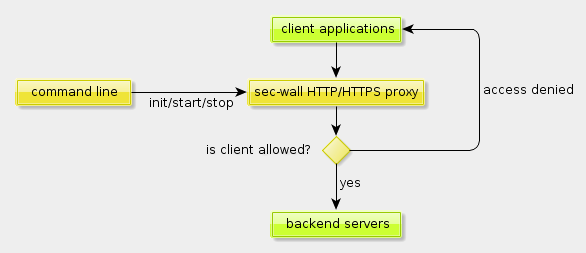
\includegraphics[width=\textwidth]{images/sec-wall-overview.png}
\end{center}
\end{frame}

\subsection{Advanced Python SOA Consumers}

\begin{frame}
\begin{center}
 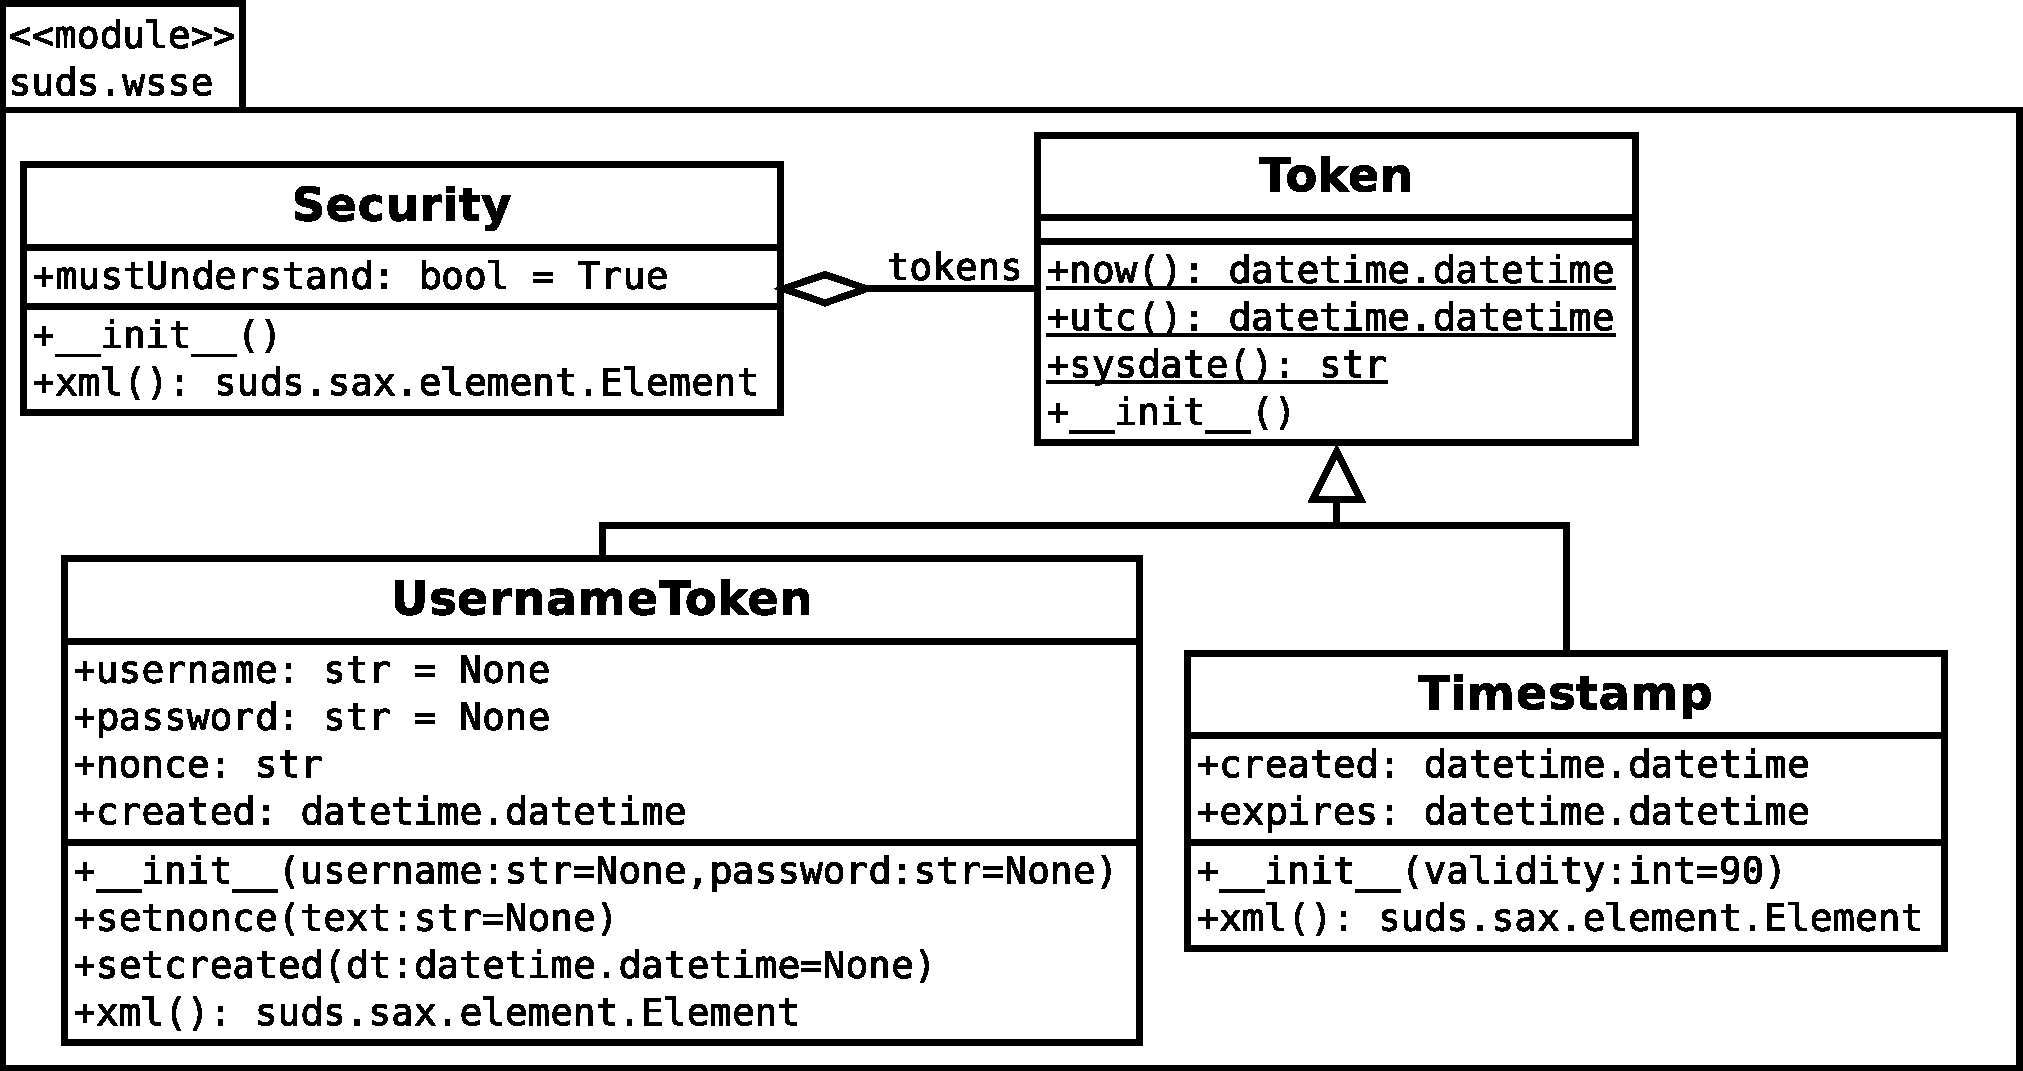
\includegraphics[width=\textwidth]{images/clsdSudsWsse.pdf}
\end{center}
\end{frame}

\section{Solution}

\subsection{UsernameToken patch}

\begin{frame}[fragile]
\begin{lstlisting}[basicstyle=\footnotesize\ttfamily]
<soap:Envelope xmlns:soap="http://schemas.xmlsoap.org/soap/envelope/">
 <soap:Header>
  <wsse:Security xmlns:wsse="..." xmlns:wsu="..." soap:mustUnderstand="1">
   <wsse:UsernameToken wsu:Id="UsernameToken-3">
    <wsse:Username>admin</wsse:Username>
    <wsse:Password Type="...#PasswordDigest">fTI7fNcwD69Z3dOT1bYfvSbQPb8=</wsse:Password>
    <wsse:Nonce EncodingType="...#Base64Binary">1DLfpq3fLJ5O8Dlrnr4blQ==</wsse:Nonce>
    <wsu:Created>2011-05-05T17:20:22.319Z</wsu:Created>
   </wsse:UsernameToken>
  </wsse:Security>
 </soap:Header>
 <soap:Body>
  ...
 </soap:Body>
</soap:Envelope>
\end{lstlisting}
\end{frame}

\subsection{SudsSigner}

\begin{frame}
\begin{center}
 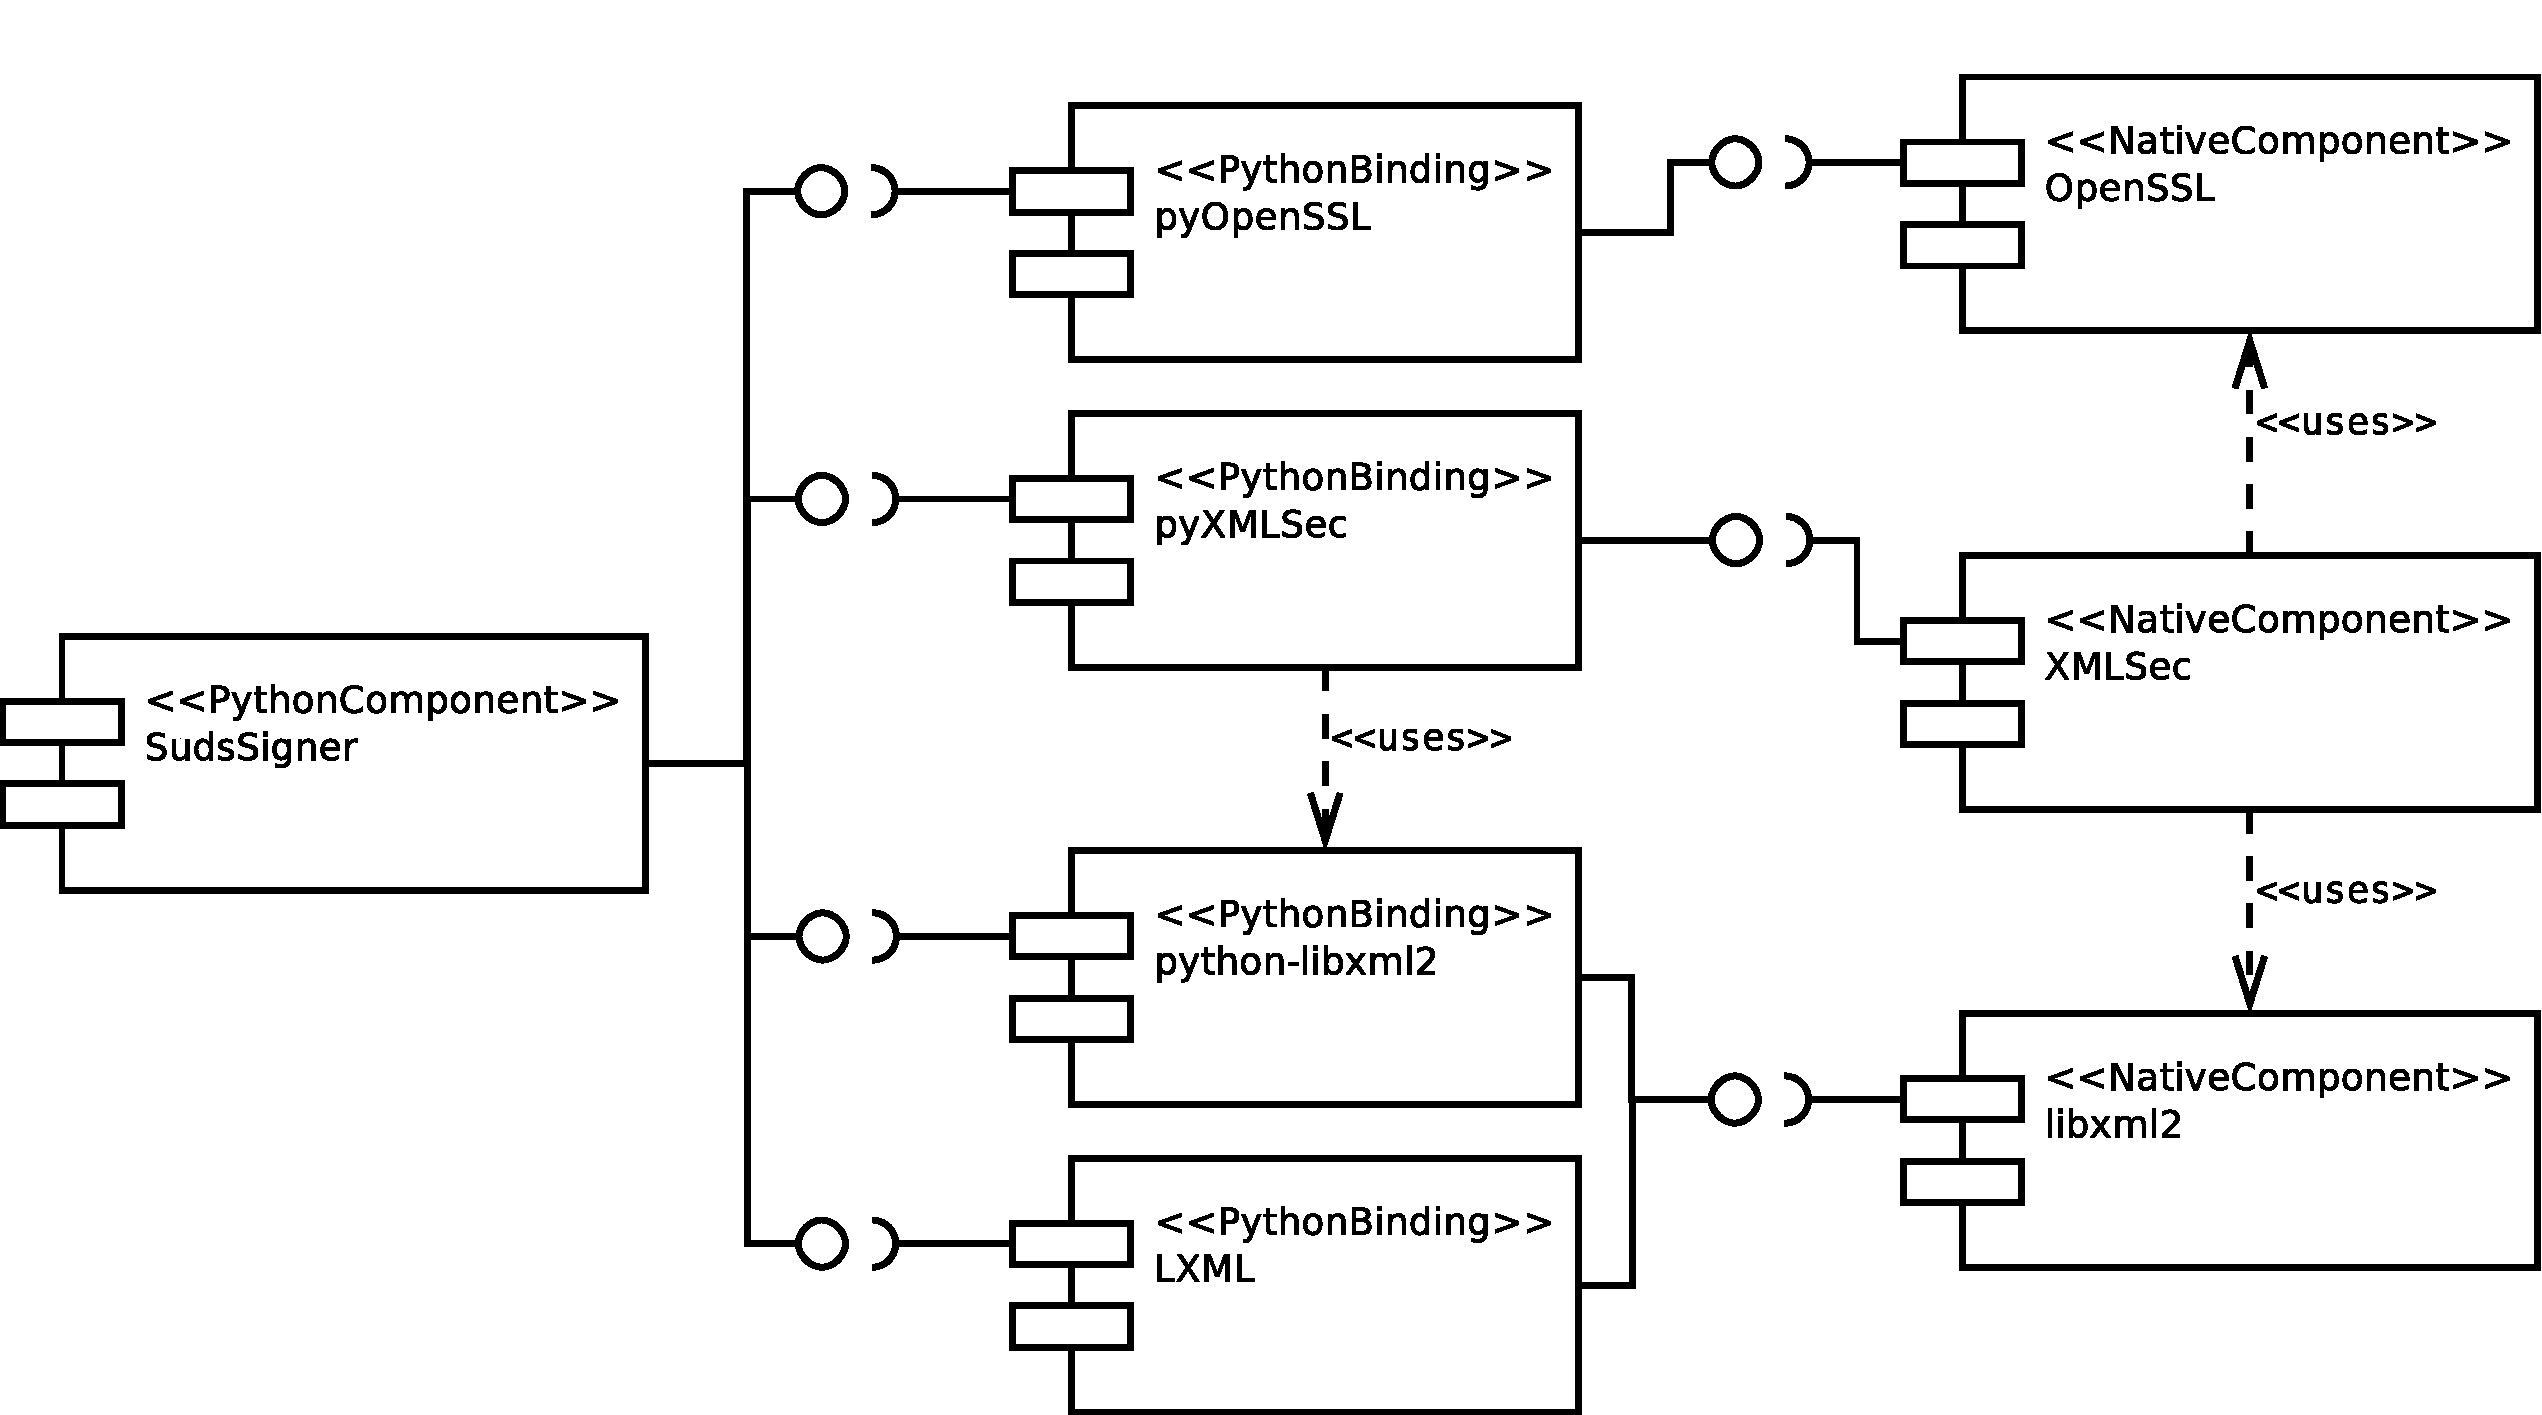
\includegraphics[width=\textwidth]{images/cmpdSudsSigner.pdf}
\end{center}
\end{frame}

\section{Results}

\subsection{Usage example}

\begin{frame}[fragile]
\begin{lstlisting}
from suds import client
from suds.wsse import Security, Timestamp
from SudsSigner.plugin import SignerPlugin

sp = SignerPlugin('privkey.pem')
c = client.Client('http://vsza.hu/foo.wsdl', plugins=[sp])

security = Security()
security.tokens.append(Timestamp())
c.set_options(wsse = security)

print c.service.say_hello('World', 3)
\end{lstlisting}
\end{frame}

\subsection{Performance}

\begin{frame}
\begin{center}
Configuration: Signed Message with Timestamp
\end{center}
\begin{table}[htbp]
 \begin{center}
    \tikzstyle barchart=[fill=black!20,draw=black]
  \tikzstyle errorbar=[very thin,draw=black!75]
  \tikzstyle scale=[very thin,draw=black!75]
  \begin{tabular}{ l l r@{.}l l }\toprule
 n & Library & \multicolumn{2}{l}{Invoke $\pm$ 1 ms} & \\
 \midrule
  1 & CXF & 1072&80 $\pm$ 50.63 &
  \begin{minipage}[c]{4cm}
   \begin{tikzpicture}
    \draw (0cm,0cm) (4,0.5);
    \draw[barchart] (0,0.152) rectangle (3.413,0.438);
    \draw[errorbar] (3.252,0.295) -- (3.575,0.295);
    \draw[errorbar] (3.252,0.333) -- (3.252,0.258);
    \draw[errorbar] (3.575,0.333) -- (3.575,0.258);
    \draw[scale] (0,0) node[] {};
   \end{tikzpicture}
  \end{minipage} \\
  1 & SUDS & 525&52 $\pm$ 49.45 &
  \begin{minipage}[c]{4cm}
   \begin{tikzpicture}
    \draw (0cm,0cm) (4,0.5);
    \draw[barchart] (0,0.152) rectangle (1.672,0.438);
    \draw[errorbar] (1.515,0.295) -- (1.829,0.295);
    \draw[errorbar] (1.515,0.333) -- (1.515,0.258);
    \draw[errorbar] (1.829,0.333) -- (1.829,0.258);
    \draw[scale] (0,0) node[] {};
   \end{tikzpicture}
  \end{minipage} \\
  10 & CXF & 133&26 $\pm$ 3.06 &
  \begin{minipage}[c]{4cm}
   \begin{tikzpicture}
    \draw (0cm,0cm) (4,0.5);
    \draw[barchart] (0,0.152) rectangle (0.424,0.438);
    \draw[errorbar] (0.414,0.295) -- (0.434,0.295);
    \draw[errorbar] (0.414,0.333) -- (0.414,0.258);
    \draw[errorbar] (0.434,0.333) -- (0.434,0.258);
    \draw[scale] (0,0) node[] {};
   \end{tikzpicture}
  \end{minipage} \\
  10 & SUDS & 80&92 $\pm$ 3.21 &
  \begin{minipage}[c]{4cm}
   \begin{tikzpicture}
    \draw (0cm,0cm) (4,0.5);
    \draw[barchart] (0,0.152) rectangle (0.257,0.438);
    \draw[errorbar] (0.247,0.295) -- (0.268,0.295);
    \draw[errorbar] (0.247,0.333) -- (0.247,0.258);
    \draw[errorbar] (0.268,0.333) -- (0.268,0.258);
    \draw[scale] (0,0) node[] {};
   \end{tikzpicture}
  \end{minipage} \\
  100 & CXF & 35&30 $\pm$ 0.30 &
  \begin{minipage}[c]{4cm}
   \begin{tikzpicture}
    \draw (0cm,0cm) (4,0.5);
    \draw[barchart] (0,0.152) rectangle (0.112,0.438);
    \draw[errorbar] (0.111,0.295) -- (0.113,0.295);
    \draw[errorbar] (0.111,0.333) -- (0.111,0.258);
    \draw[errorbar] (0.113,0.333) -- (0.113,0.258);
    \draw[scale] (0,0) node[] {};
   \end{tikzpicture}
  \end{minipage} \\
  100 & SUDS & 32&19 $\pm$ 0.46 &
  \begin{minipage}[c]{4cm}
   \begin{tikzpicture}
    \draw (0cm,0cm) (4,0.5);
    \draw[barchart] (0,0.152) rectangle (0.102,0.438);
    \draw[errorbar] (0.101,0.295) -- (0.104,0.295);
    \draw[errorbar] (0.101,0.333) -- (0.101,0.258);
    \draw[errorbar] (0.104,0.333) -- (0.104,0.258);
    \draw[scale] (0,0) node[] {};
   \end{tikzpicture}
  \end{minipage} \\
 \multicolumn{4}{l}{} &  \begin{minipage}[c]{4cm}
   \begin{tikzpicture}
    \draw (0cm,0cm) (4,0.3);
    \draw[scale] (0,0.2) -- (3.500,0.2);
    \draw[scale] (0.875,0.2) -- (0.875,0.3);
    \draw[scale] (0.875,-0.15) node[text width=0pt, text height=0pt, font=\footnotesize] {275};
    \draw[scale] (1.75,0.2) -- (1.75,0.3);
    \draw[scale] (1.75,-0.15) node[text width=0pt, text height=0pt, font=\footnotesize] {550};
    \draw[scale] (2.625,0.2) -- (2.625,0.3);
    \draw[scale] (2.625,-0.15) node[text width=0pt, text height=0pt, font=\footnotesize] {825};
    \draw[scale] (3.5,0.2) -- (3.5,0.3);
    \draw[scale] (3.5,-0.15) node[text width=0pt, text height=0pt, font=\footnotesize] {1100};
   \end{tikzpicture}
  \end{minipage} \\
  \bottomrule
  \end{tabular}

 \end{center}
\end{table}
\end{frame}

\section{}

\begin{frame}
\begin{center}
\begin{LARGE}
Thanks for your attention!
\end{LARGE}
\end{center}
\end{frame}

\end{document}
